\documentclass[times, 10pt,twocolumn]{article} 
\usepackage{latex8}
\usepackage{times}
\usepackage{graphicx}


\usepackage{stmaryrd, latexsym, amsmath, amssymb, wasysym}
\usepackage{semantic}
\usepackage{fancyvrb}

% program text
\newcommand{\cod}[1]{\mathtt{#1}}


% security type with index
\newcommand{\sts}[1]{s_{#1}^{\mathbb{L}}}
% security type without index
\newcommand{\st}{s^{\mathbb{L}}}


% symbol of constraint IS
\newcommand{\is}{\sim}
% symbol of gconstraint
\newcommand{\guard}{\lhd}
\newcommand{\sleql}{\LHD}
\newcommand{\lleqs}{\preceq}
% tag constraint
\newcommand{\tagup}{\uparrow}
% declassification constraint
\newcommand{\decl}{\downarrow}
% lifting function
\newcommand{\lift}{\nearrow}
% basic type without index
\newcommand{\typ}{\tau}
% basic type with index
\newcommand{\typn}[1]{\tau_{#1}}
% result of type system
\newcommand{\res}[2]{{#1}\mid {#2}}
% prove symbol
\newcommand{\proves}{\ensuremath{\vdash}}
% arrow combinator
\newcommand{\arrowop}[1]{$#1\negthickspace #1\negthickspace #1$}


% security label
\newcommand{\slabel}[1]{$\cod{#1}$}

% if-then-else
\newcommand{\ifthenelse}[3]{\cod{if}~#1~\cod{then}~#2~\cod{else}~#3}

% config of ArrowRef commands
\newcommand{\llocal}{\langle\hspace{-2.4 pt}|}
\newcommand{\rlocal}{|\hspace{-2.4 pt}\rangle}
\newcommand{\config}[2]{\llocal #1,#2 \rlocal}



\begin{document}
\title{A Library for Secure Multi-threaded Information Flow in Haskell}
\author{Ta-chung Tsai \qquad Alejandro Russo \qquad John Hughes \\
Department of Computer Science and Engineering\\
Chalmers University of Technology\\
412 96 G\"{o}teborg, Sweden
}


\maketitle


\begin{abstract}
Li and Zdancewic have recently proposed an approach  
to provide information-flow security via a library rather 
than producing a new language from the scratch. They show how to 
implement such a library in Haskell by using arrow combinators.
However, their approach only 
works with computations that have no side-effects. In fact, they 
leave as an open question how their library, and the mechanisms 
in it, need to be modified to consider side-effects. Another 
absent feature in the library is support for multithreaded 
programs. Information-flow in multithreaded programs still remains
an open challenge, and no support for that has been implemented 
yet. In this light, it is not surprising that the two main stream 
compilers that provide information-flow security, Jif and FlowCaml, 
lack support for multithreading. 

Following ideas taken from literature, this paper presents an extension 
to Li and Zdancewic's library that provides information-flow security in
presence of reference manipulation and multithreaded programs. 
Moreover, an online-shopping case study has been implemented to evaluate the proposed
techniques. The case study reveals that exploiting concurrency to
leak secrets is feasible and dangerous in practice. 
To the best of our knowledge, this is the first implemented tool to guarantee 
information-flow security in concurrent programs and the first implementation
of a case study that involves concurrency and information-flow policies. 
\end{abstract}


\section{Introduction}

Language-based information flow security aims to guarantee that
programs do not leak confidential data, by some form of static
analysis which rejects programs that would leak, before they are run.
Over the years, a great many such systems have been presented,
supporting a wide variety of programming constructs
\cite{Sabelfeld:Myers:JSAC}. However, the impact on programming
practice has been rather limited.

One possible reason is that most systems are presented in the context
of a simple, elegant, and minimal language, with a well-defined
semantics to make proofs of soundness possible. Yet such systems
cannot immediately be adopted by programmers---they must first be
embedded in a real programming language with a real compiler, which is
a major task in its own right. Only two such languages have been
developed---Jif \cite{Myers:POPL99,jif} (based on Java) and FlowCaml
\cite{Pottier:Simonet:POPL02,simonet03flow} (based on Caml).

Yet when a system implementor chooses a programming language,
information flow security is only one factor among many. While Jif or
FlowCaml might offer the desired security guarantees, they may be
unsuitable for other reasons, and thus not adopted. This motivated Li
and Zdancewic to propose an alternative approach, whereby information
flow security is provided via a {\em library} in an existing
programming language \cite{LiZdancewic:CSFW06}. Constructing such a library
is a much simpler task than designing and implementing a new
programming language, and moreover leaves system implementors free to
choose any language for which such a library exists.

Li and Zdancewic showed how to construct such a library for the
functional programming language Haskell. The library provides an
abstract type of secure programs, which are composed from underlying
Haskell functions using operators that impose information-flow
constraints. Secure programs are {\em certified}, by checking that all
constraints are satisfied, before the underlying functions are
invoked---thus guaranteeing that no secret information leaks. While
secure programs are a little more awkward to write than ordinary
Haskell functions, Li and Zdancewic argue that typically only a small
part of a system need manipulate secret data---for example, an
authentication module---and only this part need be programmed using
their library.

However, Li and Zdancewic's library does impose quite severe
restrictions on what a secure program fragment may do. In particular,
these fragments may have no effects of any sort, since the library
only tracks information flow through the inputs and outputs of each
fragment. While absence of side-effects can be guaranteed in Haskell
(via the type system), this is still a strong restriction. Our purpose
in this paper is to show that the same idea can be applied to support
secure programs with a much richer set of effects---namely updateable
references in the presence of (cooperative) concurrency. The
underlying methods we use---an information-flow type-system for
references, a restriction on the scheduler---are taken from the
literature; what we show here is how to {\em implement} them for a
real programming language following Li and Zdancewic's approach.

The rest of this paper is structured as follows. In the next section
we explain Li and Zdancewic's approach in more detail. One restriction
of their approach is that data-structures are assigned a {\em single}
security level---so if any part of the output of a secure program is
secret, then the entire output must be classified as secret. We need
to lift this restriction in our work, allowing data-structures with
mixed security levels, and in Section \ref{sec:refining-types} we show
how. This enables us to add references in Section
\ref{sec:adding-references}. 
%In Section \ref{sec:atm} we take a case
%study programmed in Jif, involving an ATM communicating with a bank,
%and show that it can be reprogrammed in Haskell using our library. 
We
then introduce concurrency, reviewing approaches to secure information
flow in this context in Section \ref{sec:concurrency}, in particular
ways to close the {\em internal timing} covert channel, and in Section
\ref{sec:implementing-concurrency} we describe the implementation of
our chosen approach. In Section \ref{sec:online-shopping} we present a
concurrent case study involving online shopping. With no
countermeasures, an attack based on internal timing leaks can obtain a
credit-card number with high probability in about two minutes. We
show that our library successfully defends against this
attack. Finally, in Section \ref{sec:conclusions}, we draw our
conclusions.

\section{Encoding Information Flow in Haskell} \label{sec:encodingIF}

\begin{figure}
\begin{center}
\begin{tabular}{c}
\includegraphics{puref.eps}\\
{\tt pure f}\\
\\
\includegraphics{fcompg.eps}\\
{\tt f >>> g}\\
\\
\includegraphics{fpairg.eps}\\
{\tt f***g}
\end{tabular}
\caption{Basic arrow combinators.} \label{fig:arrows}
\end{center}
\end{figure}

Li and Zdancewic's approach represents secure program fragments as {\em
  arrows} in Haskell \cite{hughes00generalising}. Arrows can be visualised as
dataflow networks, mapping inputs on the left to outputs on the right.
Arrows are constructed from Haskell functions using combinators, of
which the most important are illustrated in Figure
\ref{fig:arrows}---\verb!pure! converts a Haskell function to an
arrow, \verb!(>>>)! sequences two arrows, and \verb!(***)! pairs
arrows together. Any required left-to-right static dataflow can be
implemented using these combinators---for example, an arrow that
computes the average of a list could be constructed as
\begin{Verbatim}[fontsize=\footnotesize]
squareA = pure tee >>> 
          (pure sum *** pure length) >>> 
          pure divide
  where tee x = (x,x)
        divide (x,y) = x/y
\end{Verbatim}
\begin{figure}
\begin{center}
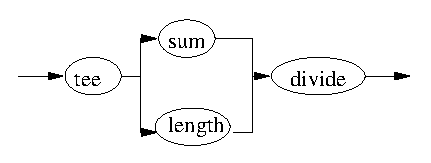
\includegraphics{average.eps}
\end{center}
\caption{Average of a list.} \label{fig:average}
\end{figure}
Its effect is illustrated in Figure~\ref{fig:average}.
To express a dynamic choice between two arrows, there is an additional
combinator \verb!f|||g!, whose input is of Haskell's sum type:
\begin{Verbatim}[fontsize=\footnotesize]
data Either a b = Left a | Right b
\end{Verbatim}
Its effect is illustrated in Figure \ref{fig:choice}.
\begin{figure}
\begin{center}
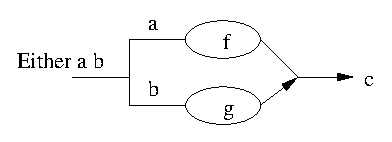
\includegraphics{choice.eps}
\caption{Choice between {\tt f} and {\tt g}.} \label{fig:choice}
\end{center}
\end{figure}

Haskell allows any suitable type to be declared to be an arrow, by
providing implementations for the basic arrow combinators. This is
usually used to encapsulate some kind of effects. For example, we
might define an arrow for programming with references, by declaring
\verb!ArrowRef a b! to be the type of arrows from \verb!a!  to
\verb!b!, implementing the basic combinators, and then providing
arrows
\begin{Verbatim}[fontsize=\footnotesize]
createRefA :: ArrowRef a (Ref a)
readRefA   :: ArrowRef (Ref a) a
writeRefA  :: ArrowRef (Ref a,a) ()
\end{Verbatim}
to perform the basic operations on references. With these definitions,
we can write side-effecting programs in a dataflow style. For example,
an arrow to increment the contents of a reference could be programmed
as
\begin{Verbatim}[fontsize=\footnotesize]
incrRefA :: ArrowRef (Ref Int) ()
incrRefA = 
  (pure id &&& (readRefA >>> pure (+1)))
  >>> writeRefA
  where f &&& g = pure tee >>> (f***g)
\end{Verbatim}

Li and Zdancewic found another use for arrows: they realised that,
since all the data- and control-flow in an arrow program is expressed
using the arrow combinators, then they could define a type of {\em
  flow arrows}, whose primitive arrow combinators implement the type
checking of an information flow type system.  Their type system
assigns a {\em security label} drawn from a suitable lattice, such as
\begin{Verbatim}[fontsize=\footnotesize]
data Label = LOW | MEDIUM | HIGH
  deriving (Eq, Ord)
\end{Verbatim}
to the input and output of each arrow (where the \verb!deriving!
clause declares that \verb!LOW!$\leq$\verb!MEDIUM!$\leq$\verb!HIGH!).
Their arrows themselves are represented by the type 
%
\verb!FlowArrow l arr a b!, 
%
which is actually an {\em arrow transformer}: the type \verb!l! is the
security lattice, \verb!a! and \verb!b! are the input and output
types, and \verb!arr! is an {\em underlying arrow} type such as
\verb!ArrowRef!. Flow arrows {\em contain} arrows of type 
%
\verb!arr a b!, together with flow information about their inputs and
outputs.

In the information flow type system, an arrow is assigned a flow type
$\ell_1\rightarrow\ell_2$ under a set of constraints, where $\ell_1$ and
$\ell_2$ are security labels. The rules for \verb!pure! and \verb!(>>>)!
are given in Figure \ref{fig:basic-rules}.
\begin{figure}
{\small
\[
\inference[]{}{ \proves \mbox{\tt pure}~f : \ell \rightarrow \ell}
\quad
\inference[]{C_1\proves f:\ell_1\rightarrow \ell_2\quad C_2\proves g:\ell_3\rightarrow \ell_4
  }{C_1, C_2, \ell_2\sqsubseteq \ell_3 \proves f\mbox{\tt >>>}g : \ell_1\rightarrow \ell_4}
\]
}
\caption{Typing rules for {\tt pure} and {\tt >>>}.} \label{fig:basic-rules}
\vspace{-10pt}
\end{figure}
The \verb!FlowArrow! type represents not only the underlying
computation, but also the information flow typing---it is represented
as a record
\begin{Verbatim}[fontsize=\footnotesize]
data FlowArrow l arr a b = FA
  { computation :: arr a b,
    flow        :: Flow l,
    constraints :: [Constraint l]
  }
data Flow l = Trans l l | Flat
data Constraint l = LEQ l l
\end{Verbatim}
Here the \verb!flow! component represents either
$\ell_1\rightarrow\ell_2$ (\verb!Trans l1 l2!), or the ``polymorphic''
$\ell\rightarrow \ell$ for any $\ell$ (\verb!Flat!), which is needed to give an
accurate typing for \verb!pure!. The \verb!constraints! field just
collects the constraints on the left of the turnstile. With this
representation, it is easy to implement the typing rules in the arrow
combinators. Security labels are introduced and checked by the arrow
\verb!tag l!, with flow \verb!Trans l l!, which forces both its input
and output to have the given security label.

Note that the information flow types are quite independent of the
Haskell types! Moreover, they are not checked during Haskell
type-checking. Rather, when a flow arrow is constructed during program
execution, all the necessary constraints are collected
dynamically---but they are checked before the underlying computation
is run. Li and Zdancewic's library exports \verb!FlowArrow! as an
abstract type, and the only way to extract the underlying computation
is via a certification function which solves the constraints first. If
any constraint is not satisfied, then the underlying code is rejected.

Li and Zdancewic also considered declassification, which requires
adding the user's security level as a context to the typing rules, and
a new form of constraint---but we ignore the details here.



\section{Refining Security Types} \label{sec:refining-types}

%pure problem, lowerA
% todo : define data TwoLabel = HIGH | LOW or other lattice label

Li and Zdancewic's library uses single security labels as 
security types. As a consequence, values are classified 
secrets when they contain, partially or totally, some 
confidential information. For instance, if one component of a pair is
secret, the whole pair becomes confidential. This design 
decision might be a potential restriction to build some applications 
in practice. With this in mind, we  extend 
Li and Zdancewic's work to include security types with more than one security
label. The presence of several security labels 
in security types allows to develop a more precise, and consequently
permissive, analysis of the information flow inside of a program. 

%Once they form a pair of integers, the integer protected by $\cod{LOW}$ is lifted to $\cod{HIGH}$.
%This might be a potential restriction in real-world applications.
%Thus, we first extend their work by introducing extended security types that
%support precise description of data. With this new security types, sub-components
%of complex data can be protected by different security labels.

\subsection{Security Types} \label{sec:extendedST}

We assume a given security lattice $\mathbb{L}$ where 
security levels, denoted by $\ell$, are ordered by
a partial order $\leq$. Top and bottom elements are 
written $\top$ and $\bot$, respectively. 
%The top and bottom
%elements of this lattice  are respectively noted as $\top$ and $\bottom$.
\begin{figure}
{\small{
\[
\st\ ::=\ \ell\ |\ (\st,\st)\ |\ ({\mathbf{either}}\ \st\ \st\ )^{\ell}\
\]
\caption{\label{fig:extendedST} Extended security types}
}}
\end{figure}
%
%
\begin{figure}[]
{\small{
\[
 \begin{array}{c}
   \inference[]{\ell_1 \leq \ell_2}{\ell_1 \sqsubseteq \ell_2} \quad
   %\inference[]{\sts{1}=\sts{2} \quad \ell_1 \sqsubseteq \ell_2}
   %            {\sts{1}\ \mathbf{ref}^{\ell_1} \sqsubseteq \sts{2}\ \mathbf{ref}^{\ell_2}} \quad
   \inference[]{\sts{1} \sqsubseteq \sts{3} \quad \sts{2} \sqsubseteq \sts{4} }
               {(\sts{1},\sts{2}) \sqsubseteq (\sts{3},\sts{4})} \\ \\
   \inference[]{\ell_1 \sqsubseteq \ell_2 \quad \sts{1} \sqsubseteq \sts{3} \quad \sts{2} \sqsubseteq \sts{4}}
               {(\mathbf{either}\ \sts{1}\ \sts{2})^{\ell_1} \sqsubseteq
                (\mathbf{either}\ \sts{3}\ \sts{4})^{\ell_2} } \\
 \end{array}
\]
\caption{\label{fig:subtyping} Subtyping relationship}
}}
\vspace{-10pt}
\end{figure}
Security
types are given in Figure \ref{fig:extendedST} and their subtyping
relationship in Figure \ref{fig:subtyping}. Security
type $(\st,\st)$ provides security annotations for 
pair types.  %, e.g. $\texttt{(Int,Float)}$. 
Security type $({\mathbf{either}}\ \st\ \st\ )^{\ell}$ provides
annotations for type $\texttt{Either}$.
%Types $\texttt{a}$ and $b$ are also annotated by 
%$\st_1$ and $\st_2$, respectively. Security label $\ell$ annotates 
%the constructors $\texttt{Left}$ and \texttt{Right}$. 
%avoid leakings by just looking what constructor is used to build  
%values of type $\texttt{Either a b}$. 
Security type $\ell$ decorates any other 
Haskell type (e.g. $\texttt{Int}$, $\texttt{Float}$, $\texttt{[a]}$,
etc.). Security types are represented in our library as follows:
%The representation of these types in our library is
%the following:
%Security types in Figure \ref{fig:extendedST} are implemented 
%$\texttt{SecType}$ as follows:
\begin{Verbatim}[fontsize=\footnotesize]
data SecType l 
         = SecLabel l
         | SecPair (SecType l) (SecType l) 
         | SecEither (SecType l) (SecType l) l
\end{Verbatim}
\noindent
where $\texttt{l}$ implements a lattice of security levels.

\subsection{Defining FlowArrowRef} \label{sec:flowarrowref}
The abstract data type $\cod{FlowArrowRef}$ defines our embedded
language by implementing an {\em arrow} interface:
%
\begin{Verbatim}[fontsize=\footnotesize]
data FlowArrowRef l a b c = FARef
     { computation  :: a b c
     , flow         :: Flow (SecType l)
     , constraints  :: [Constraint (SecType l)] }
\end{Verbatim}
This definition is similar to the definition of 
\texttt{FlowArrow} except for using $\texttt{(SecType l)}$
as type argument for $\texttt{Flow}$ and $\texttt{Constraint}$.
%However, with the addition of references, some new fields are required 
%in order to properly handle side-effects. The addition of these extra
%fields is differed to Section \ref{sec:adding-references}.
%
Constructor \texttt{Flat}  needs to be removed
from data type \texttt{Flow} as a consequence of dealing with security types 
with more than one security label. 
In \texttt{FlowArrow}, \texttt{Flat} 
is used to establish that pure computations have
the same input and output security type. Unfortunately, \texttt{Flat}
cannot be used in \texttt{FlowArrowRef}, otherwise secrets might be
leaked. 
For instance, consider the program 
\texttt{ pure (\ (x,y) -> (y,x) )} that just  flips 
components in a pair. Assume that \texttt{x}, annotated 
with security label \texttt{HIGH}, is a secret input and \texttt{y}, 
annotated with security label \texttt{LOW}, contains public
information. If \texttt{(HIGH,LOW)} is the input and output
security types for that program, the value of 
\texttt{x} will be immediately revealed! 
%This example aims to show that it can be
%difficult to accurately determine output security type when
%combinator \texttt{pure} is applied to more complex functions. 
%We will deal with this problem in  Section \ref{sec:pure}. 


Similarly to Li and Zdancewic's work, \texttt{FlowArrowRef}
encodes a typing judgment to verify information-flow
policies. Naturally,  our encoding is more complex than 
that in \texttt{FlowArrow}. This complexity essentially 
arises from considering richer security types.
%and side-effect, like reference manipulation, inside of arrow 
%computations. 
%Essentially, our implementation encodes a more complex 
%type checker.
%For simplicity, we introduce the typing
%judgement, but without considering side-effects produced by references.
%Later on, in Section \ref{sec:adding-references}, we will show how to
%handle them. 
The typing judgment has the form:
$
 C  \proves f~:~\res{\typn{1}}{\sts{1}}~->~\res{\typn{2}}{\sts{2}}
$, 
%
%\noindent
where $f$ is a purely-functional computation,  
$C$ is a set of constrains
that, when satisfied, guarantees information-flow policies, and 
$\res{\typn{1}}{\sts{1}}~->~\res{\typn{2}}{\sts{2}}\ \ $ is a \emph{flow
  type}, which denotes
that $f$ receives  input values of type $\tau_1$ with
security type $\sts{1}$, and produces output values of type
$\tau_2$ with security type $\sts{2}$. Except for 
combinator \texttt{pure}, 
most of the typing rules in 
Li and Zdancewic's work can be easily rewritten using this 
typing judgement, and therefore, we omit them here. 

% that involves unification. 
%Unification is needed to 
%pass around more detailed information  
%Unification is needed in 
%order to relief programmers of frequently indicating security labels 
%when create computations
%Unification is not present 
%is Li and Zdancewic's library since they security type  considering only 
%
%An interesting aspect of 
%implementing unification by arrows is dealing with renaming.  
%   
%Consequently, programmers are relief of 
%indicating security labels when they can be inferred from the context.






%n data type $\cod{Flow}$, constructor $\cod{Flat}$ is removed because it loses 
%structure information of security types. New constraint type $\cod{GConstraint}$ represents
%constraints related to a security type and a security label. It differs from $\cod{Constraint}$
%which involves two security types. 
%Field $\cod{pc}$ keeps track of the lower bound of side effects in a computation, while
%field $\cod{purep}$ records whether a computation is only constructed by $\cod{pure}$ computations. 
%The purposes of these two fields are further explained in Sec.~\ref{sec:refpriv}.
%
%\paragraph{Type System}
%
%
%A type system is developed for combinators of $\cod{FlowArrowRef}$. 
%The following explains the type judgement and presents part of the type system.
%
%The type judgement has following form:

%Environment variable $pc$ is the lower bound of side effects produced by computation $\cod{f}$.
%Variable $\Delta$ denotes constraints of the form $\ell \guard \st$, $\st \sleql \ell$, and $\ell \lleqs \st$,
%and is implemented by data type $\cod{GConstraint}$.
%Constraint $\ell \guard \st$, read ``$\ell$ guards $\st$'', is defined in terms of function $e$, as in
%Fig.~\ref{fig:flowarrowref:guard}.
%Function $e$, defined in Fig.~\ref{fig:extract}, extracts a security label from a security type which 
%represents the security level of the security type. 
% todo : do I need further explain?
%Constraint $\st \sleql \ell$ requires the highest security label in $\st$ is lower than or equal to $\ell$,
%while constraint $\ell \lleqs \st$ requires the lowest security label in $\st$ is higher than or equal to $\ell$.
% todo : should I mention mext_join & mext_meet?
%Variable $\Theta$ represents constraints of the form $\st \sqsubseteq \st$, $\st \sqsubseteq \cod{user}$,
%and $\st \is \st$, and is implemented by data type $\cod{Constraint}$.
%Constraint $\sqsubseteq$ is defined according to the sub-typing relation in Fig.~\ref{fig:subtyping}.
%Constraint $\st \is \st$ requires two security types have the same structure.
%Variable $\Pi$ is $\cod{T}$ if the computation is only built from $\cod{pure}$s, and $\cod{F}$, otherwise.
%The input and output types of computation $\cod{f}$ are $\typn{1}$ and $\typn{2}$ respectively, while
%the input and output security types of $\cod{f}$
%are $\sts{1}$ and $\sts{2}$, respectively.


\subsection{Security Types and Combinator  $\texttt{pure}$} \label{sec:pure}

%% Situation and Problem
Different from Li and Zdancewick's work, it is not 
straightforward to determine security types for computations 
built with arrow combinators. Basically, the difficulty comes from 
deciding the output security type for combinator \texttt{pure}. 
This combinator can take any arbitrary Haskell 
function as its argument. Then, the structure of its output, 
and consequently its output security type, can be different in every
application. 
For instance, output security types for \texttt{pure} computations
that return numbers and pair of numbers consist of security labels and 
pair of security labels, respectively. 
% while output security types
%for \texttt{pure} computations returning a pair of numbers are pairs of 
%security labels.
Moreover, 
although the structure of the output security
type could be determined, it is also
difficult to establish the security labels 
appearing in it. To illustrate this point, consider the 
computation 
\texttt{pure ( $\backslash$(x,y) -> (x+y, y) )}, where inputs 
$x$ and $y$ have security labels $\texttt{LOW}$ and
$\texttt{HIGH}$, respectively. 
It is clear that the output security
type for this example is $(\texttt{HIGH},
\texttt{HIGH})$. However, 
in order to determine that, it is necessary to 
know how the input is used to build the output.
This input-output dependency might be difficult to 
track when more complex functions are considered.
With this in mind, 
we introduce a new security
type to $\st$:
\[
\st\ ::=\ \ell\ |\ (\st,\st)\ |\ ({\mathbf{either}}\ \st\ \st\
)^{\ell}\ |\ \mathbf{high}
\]

% 
\begin{figure}
{\small
\[
 \inference[]{f~::~\typn{1}~->~\typn{2}}
             {\emptyset \proves \cod{pure}~f~:~
             \res{\typn{1}}{\sts{1}}~->~\res{\typn{2}}{\mathbf{high}}} 
\]
\caption{\label{fig:typingpure} Typing rule for combinator \texttt{pure}}
}
\vspace{-10pt}
\end{figure}

Security type $\mathbf{high}$ represents any security
type that contains all their security labels as $\top$. 
Typing rule for \texttt{pure} is given in Figure
\ref{fig:typingpure}. Observe the use of the Haskell 
typing judgment, written $::$, in the hypothesis of the rule. 
%We approximate 
%the output security type of \texttt{pure} by  
%$\mathbf{high}$. 
Results of \texttt{pure} computations are
thus confidential regardless
what they do or what kind of result they return.
Unfortunately,  by doing this, computations that  
follow combinator \texttt{pure} cannot operate on 
public data any more. As an example, consider the 
program 
%following piece of code that only operates on public information: 
%\begin{Verbatim}[fontsize=\footnotesize]
\texttt{f >>> pure ( $\backslash$x -> x + 1) >>> g},
%\end{Verbatim}
where \texttt{f} and \texttt{g} 
operate on public data. This simple program just adds one to the
public output of \texttt{f} and provides that as the input of \texttt{g}. However, 
the program is rejected by the encoded type system in our library, even
though no leaks are produced by this code. 
%Observe that 
%computation 
The reason for this is that program \texttt{g} receives confidential information
from \texttt{pure} while it expects only public inputs. 
%, it
% receives confidential information from combinator
%\texttt{pure}. 
%Therefore, the encoded type system reject according to the encoded type
%system in \texttt{FlowArrowRef},  a leak might happen. 
Since \texttt{pure} is responsible for
allowing the use of any Haskell functions in the library, this restriction seems to be quite 
severe to implement concrete applications. 
%In order to overcome it, a new combinator is defined in the next section.

\subsection{Combinator $\cod{lowerA}$} \label{sec:lowerA}
Combinator \texttt{lowerA} is introduced to mitigate the restriction 
of not allowing computations on public data to take some input
produced by $\cod{pure}$ combinators. Basically, \texttt{lowerA}
takes a security label $\ell$ and an arrow computation $p$, 
and returns a computation $p'$. Computation $p'$ behaves 
like $p$ and has the 
same input type, output type, and input security type as $p$. However, 
its output security type might be different. The output security 
type is constructed based on the output type of $p$ and it 
contains only security labels of value $\ell$. 
%termined based on the output type of $p$ 
%and it constains 
%$\ell$ as the only security labels appearing in it. 
In other words, \texttt{lowerA} downgrades the output of $p$ 
to the security level $\ell$. In principle, this combinator 
might be also used to leak secrets. 
An attacker can just apply \texttt{(lowerA LOW)} to every computation 
that involves secrets! To avoid this kind of attacks, 
\texttt{lowerA} filters out data with
security level higher than $\ell$. 

%To put it briefly, \texttt{lowerA}
%wraps computation $p$ with mechanism, based on type-classes, to filter 
%out data and to build security types with only one security label.


\subsubsection*{Input Filtering Mechanism}

Filtration of data is done by replacing some pieces of
information with \texttt{undefined}
\footnote{This is an undefined value in Haskell
  and it is member of every type.}. 
This idea is implemented by the function \texttt{removeData} of the
type-class \texttt{FilterData}. 
The signature of the type-class is the
following:
\begin{Verbatim}[fontsize=\footnotesize]
class (Lattice l) => FilterData l t where
  removeData :: l -> t -> (SecType l) -> t
\end{Verbatim}
%Basically,  mechanism takes 
%a security label $\ell$, a value $v$ of type $\tau$, and a security 
%type $\st$ as arguments, and produces another value of type $\tau$
%but where only the information
%with security level higher than $\ell$ was changed by \texttt{undefined}.  

Method \texttt{removeData} receives a security level $\texttt{l}$, 
a value of type \texttt{t}, and a security type
\texttt{(SecType l)}, and produces another value of type \texttt{t} where 
the information with security label higher than \texttt{l} is 
replaced by \texttt{undefined}. 
As an example, instantiations for 
integers and pairs are given in Figure \ref{fig:FilterData}. 
Observe how the use of type-classes 
allows to define different filtering policies for different kind 
of data. This is particularly useful when references are introduced 
in the language (see Section \ref{sec:proyections}).  

\begin{figure}
\begin{Verbatim}[fontsize=\footnotesize]
instance (Lattice l) 
         => FilterData l Int where
            removeData l x (SecLabel l') =
             if label_leq l' l then x 
             else undefined
instance (Lattice l, FilterData l a, 
          FilterData l b) 
          => FilterData l (a,b) where
          removeData l (x, y) (SecPair lx ly) =
            (removeData l x lx, removeData l y ly)
\end{Verbatim}
\caption{\label{fig:FilterData}Instantiations for \texttt{FilterData}}
\end{figure}
%The instance for integers returns \texttt{undefined}
%if the security label of the information to filter out, \texttt{l'}, 
%is higher than \texttt{l}.
%In the instance for pairs, $\cod{removeData}$ is applied recursively to both components
%of the pair with their corresponding values and security types.

\subsubsection*{Building Output Security Types}

\begin{figure}[t]
\begin{Verbatim}[fontsize=\footnotesize]
instance (Lattice l) => 
         BuildSecType l Int where
         buildSecType l _ = (SecLabel l)

instance 
 (Lattice l, BuildSecType l a, BuildSecType l b) 
 => BuildSecType l (a,b) where
    buildSecType l _ = 
        (SecPair (buildSecType l (undefined::a)) 
                 (buildSecType l (undefined::b)))
\end{Verbatim}
\caption{\label{fig:BuildSecType}Instantiations for \texttt{BuildSecType}}
\vspace{-10pt}
\end{figure}

\begin{figure}[t]
\begin{Verbatim}[fontsize=\footnotesize]
instance 
 (Lattice l, BuildSecType l c, Arrow a) 
 => TakeOutputType l a b c where
 deriveSecType l ar = 
    buildSecType l (undefined::c)
\end{Verbatim}
\caption{\label{fig:TakeOutputType}Instantiation for \texttt{TakeOutputType}}
\end{figure}


Besides introducing a filtering mechanism, \texttt{lowerA} 
constructs output security types where security labels are all 
the same.
We define the following
type-class:
%Method $\cod{buildSecType}$ 
%in type-class \texttt{BuildSecType} implements this idea. 
%The signature for this type-class is the following:
\begin{Verbatim}[fontsize=\footnotesize]
class (Lattice l) => BuildSecType l t where
  buildSecType :: l -> t -> (SecType l)
\end{Verbatim}

Method $\cod{buildSecType}$ receives a security label \texttt{l} and 
a value of type \texttt{t}, and produces a  
security type for \texttt{t} where security labels are \texttt{l}. 
For instance, it produces 
security type \texttt{(l,l)} for pair of integers. 
Instantiations for pairs and integers are given in Figure 
\ref{fig:BuildSecType}.  Observe that the value of 
the second argument of \texttt{buildSecType} is not needed, but its type. 
Type-classes provide a mechanism to access information 
about types in Haskell and take different actions, like building different
security types, depending on them.

When \texttt{lowerA} receives a computation as an argument, it 
needs to know its output type in order to properly apply
\texttt{buildSecType}. For that purpose, we introduce another type-class:
\begin{Verbatim}[fontsize=\footnotesize]
class (Lattice l, Arrow a) 
       => TakeOutputType l a b c where
       deriveSecType :: l -> (a b c) -> (SecType l)
\end{Verbatim}
Method \texttt{deriveSecType} receives a security label \texttt{l},
an arrow computation \texttt{(a b c)}, and returns the corresponding 
security type \texttt{(SecType l)} for the output type
\texttt{c}. The instantiation of this type-class is shown in Figure 
\ref{fig:TakeOutputType}. 


%Observe how the use of \emph{lazy pattern matching} in 
%the instances of \texttt{buildSecType} allows 
%to pass an \texttt{undefined} value as argument and 
%builds the appropriate security type.


\begin{figure}[t]
\begin{Verbatim}[fontsize=\footnotesize]
lowerA :: ( Lattice l, Arrow a, 
            FilterData l b, BuildSecType l c,
            TakeOutputType l 
             (FlowArrowRef l a) b c )
          => l -> FlowArrowRef l a b c -> 
             FlowArrowRef l a b c
\end{Verbatim}
\caption{\label{fig:lowerA} Type signature for \texttt{lowerA}}
\vspace{-10pt}
\end{figure}
\begin{figure}[t]
{\small{
\[
  \begin{array}{c}
    \inference[]{ C \proves f~:~
                    \res{\typn{1}}{\sts{1}}~->~\res{\typn{2}}{\sts{2}}}
                    {C \proves \cod{lowerA}~\ell~f~:~
                    \res{\typn{1}}{\sts{1}}~->~\res{\typn{2}}{\rho(\ell,\typn{2})}} \\ 
  \end{array}
\]
}}
\caption{Typing rule for \texttt{lowerA}}
\vspace{-10pt}
\label{fig:lowerA:typesystem}
\end{figure}


To put it briefly, combinator \texttt{lowerA} 
%filters out data and build output security types based on 
%output Haskell types. It 
creates a new computation that behaves as 
the computation received as argument, but 
calling the methods $\cod{removeData}$ and $\cod{buildSecType}$ in due
course. The type signature for $\cod{lowerA}$ is given in 
Figure \ref{fig:lowerA}. 
%
Typing rule for \texttt{lowerA} is shown in Figure
\ref{fig:lowerA:typesystem}. 
Observe how the output security type is changed. 
Function $\rho$ is implemented by method 
\texttt{buildSecType}, and therefore, we omit its definition.

As a simple example of the use of \texttt{lowerA},
we rewrite the example in Section \ref{sec:pure}
as follows: 
%\begin{Verbatim}[fontsize=\footnotesize]
\texttt{f >>> lowerA LOW (pure ($\backslash$x -> x + 1)) >>> g}.
%\end{Verbatim} 
Observe that the value received by program \texttt{g} is not confidential
anymore, and consequently, the program passes the type-checking tests 
in our library. 


\section{Adding References} \label{sec:adding-references}

Dealing with information-flow security in languages with reference
manipulation is not a novelty. Unsurprisingly, Jif and FlowCaml include
them as a language feature. Nevertheless, it is stated as an open
question how Li and Zdancewic's library needs to be modified to
consider side-effects. In particular, what arrows 
could be used to handle them and how their encoded type system
needs to be modified. We have already started answering these 
question with the modification of \texttt{pure} 
and the introduction of \texttt{lowerA} in Section
\ref{sec:refining-types}. 
We will complete answering Li and Zdancewic's questions 
by showing how to extend their library to introduce references.
The developed techniques in this section can be considered 
for other kind of side-effects as well.

% --- static checking for the content of a reference--why? ---
% add security type for references (invariant in sub-typing relation)
% define reference type
% lowerA with reference
% singleton types and new reference type
% reference primitives (mention unification)

\subsection{Security Types for References}
The treatment of references is based on 
Pottier and Simonet's work \cite{Pottier:Simonet:POPL02}.
They introduce security types for references containing two 
parts: a security type and a security label. The 
security type provides information about the data that 
is referred to, while the security label gives a security 
level to the reference itself as a value. 
Following the same approach, we extend our 
security types as follows:
\[
\st\ ::=\ \ell\ |\ (\st,\st)\ |\ ({\mathbf{either}}\ \st\ \st\
)^{\ell}\ |\ \mathbf{high} \ |\ \st\ \mathbf{ref}^{\ell}
\]

Observe that security types for references ($\st\
\mathbf{ref}^{\ell}$) are composed of two parts as mentioned before.
The subtyping relationship is also extended
as follows:
%\begin{figure}[t]
\begin{equation}
 \begin{array}{c}
   \inference[]{\sts{1}=\sts{2} \quad \ell_1 \sqsubseteq \ell_2}
               {\sts{1}\ \mathbf{ref}^{\ell_1} \sqsubseteq \sts{2}\ \mathbf{ref}^{\ell_2}} \quad
 \end{array}
\label{eq:subtyping-references}
\end{equation}
%\caption{Sub-typing of reference security types}
%\label{fig:subtypingref}
%\end{figure}
In order to 
avoid aliasing problems\cite{ProgramAnalysis99},
this rule imposes an invariant in the subtyping relationship by 
requiring $\st_1$ to be the same as $\st_2$. Clearly, this 
invariant needs to be preserved by the arrow combinators in the
library. However, \texttt{lowerA} could break that invariant! 
Remember that it changes every security label in the output security
type of a given computation. As a consequence, we need to modify its
implementation (see Section \ref{sec:refinlowerA}).

Data type \texttt{SecType} is extended as follows:
\begin{Verbatim}[fontsize=\footnotesize]
data SecType l 
         = SecLabel l
         | SecPair (SecType l) (SecType l)
         | SecEither (SecType l) (SecType l) l
         | SecRef (SecType l) l
\end{Verbatim}
\noindent
where \texttt{SecRef (SecType l) l} represents security types for references.

\subsection{References and Combinator $\cod{lowerA}$}
\label{sec:refinlowerA}

Combinator \texttt{lowerA} could break the subtyping invariant for
references described in $(\ref{eq:subtyping-references})$. 
As a result, aliasing
problems, and therefore leakage of secrets, might be introduced.  
The root of this problem comes from the fact that
\texttt{lowerA} only uses output types  
to determine output security types. 
To illustrate this problem, consider a program 
that has two public references, \texttt{r1} and \texttt{r2},
with security type 
\texttt{(SecRef (SecLabel LOW) LOW)}. Assume that both references
refer to the same 
value. If \texttt{r1}, for instance, is fed into the computation 
\texttt{lowerA HIGH (pure id)}, the output produced, which is 
obviously \texttt{r1}, will have security type 
\texttt{(SecRef (SecLabel HIGH) HIGH)}. Observe that the security type 
for the content of the reference has changed. After doing that, leaks can 
occur by writing secrets using \texttt{r1} and reading them out by 
using \texttt{r2}. 
Naturally, \texttt{lowerA} could also examine input 
security types, but 
unfortunately this is not enough. Once again, the 
difficulty to track input-output dependencies of \texttt{pure}
computations (see Section \ref{sec:pure}) makes it difficult to determine, 
for instance,  which reference from the input correspond 
to which reference in the output. Consequently, it 
is also difficult to determine security types for references 
in the output based on the input security types. To overcome 
this problem, we use a mechanism that can
transport security information about contents of references from
the input to the output of an arrow computation. In this way, 
\texttt{lowerA} can read this information and place
the corresponding security types
references when needed, and thus keep the subtyping invariant.
%output security type. 
This mechanism relies on the use of singleton
types, which are the topic of the next section.


\subsection{Preserving Subtyping Invariants}

On one side, combinator \texttt{lowerA} builds output security types
based on the output type of computations. 
On the other hand, security types for the content of references must
never be changed. So, why not encoding in the Haskell type system 
the security type for the content of references? 
Hence, \texttt{lowerA} can take
the encoded information and precisely determines the 
corresponding security type for the content of each reference. 

Singleton types \cite{pierce:AdvanceTypeBook} are adequate to represent specific 
values at the level of types. Essentially, they allow to have a match 
between values and types and vice versa. 
%To obtain this very fine-grained
%association, types need to be
%inhabited by only one defined value. 
Our goal is, therefore, to 
encode values of type
(\texttt{SecType l}) in more fine-grained Haskell types. For instance, 
the encoding for values of type \texttt{(SecType Label)}
%where \texttt{Label} is the three label lattice introduced 
%in Section \ref{sec:encodingIF}, 
can be done as follows:
%As security types depend on a security lattice, we need to choose 
%that parameter before producing the encoding. For simplicity, we take 
%the three label security lattice \texttt{Label} introduced in Section \ref{sec:encodingIF}.
%We firstly encode the levels in that lattice using singleton types:
%\end{Verbatim}
%Observe how types \texttt{SLow}, \texttt{SMedium}, and \texttt{SHigh}
%represent values \texttt{HIGH}, \texttt{MEDIUM}, and \texttt{LOW}, 
%respectively. Then, the encoding for security types is the following:
%\begin{Verbatim}[fontsize=\footnotesize]
\begin{Verbatim}[fontsize=\footnotesize]
data SLow    = VLow
data SMedium = VMedium
data SHigh   = VHigh

data SSecLabel  lb        = VSecLabel  lb
data SSecPair   st1 st2   = VSecPair   st1 st2
data SSecEither st1 st2 lb= VSecEither st1 st2 lb
data SSecRef    st  lb    = VSecRef    st  lb
\end{Verbatim}
Observe how one type has been introduced for each constructor appearing in 
\texttt{Label} and \texttt{SecType}. With this encoding,  
we can now represent security types in the Haskell type system. 
As an example, security type 
\texttt{(SecRef (SecLabel HIGH) LOW)} can be encoded using the 
value \texttt{(VSecRef (VSecLabel VHigh) VLow)} of type 
\texttt{(SSecRef (SSecLabel SHigh) SLow)}. %This example shows 
%the one-to-one correspondence between values and types of our encoding.

As mentioned before, \texttt{lowerA} should use the encoded 
information to place the corresponding 
security types for content of references. 
In order to achieve that, we need a mapping 
from singleton types to values
of type \texttt{(SecType l)}. The following code implements that: 

\begin{Verbatim}[fontsize=\footnotesize]
class STLabel lb l where
  toLabel :: lb -> l

instance STLabel SLow Label where
  toLabel _ = LOW
instance STLabel SMedium Label where
  toLabel _ = MEDIUM
instance STLabel SHigh Label where
  toLabel _ = HIGH

class STSecType st l where
  toSecType :: st -> SecType l

instance STLabel lb l 
  => STSecType (SSecLabel lb) l where
  toSecType _ 
    = SecLabel (toLabel (undefined::lb))
instance (STSecType st l, STLabel lb l)
  => STSecType (SSecRef st lb) l where
  toSecType _  
    = SecRef (toSecType (undefined::st)) 
             (toLabel (undefined::lb))
instance (STSecType st1 l, STSecType st2 l)
  => STSecType (SSecPair st1 st2) l where
  toSecType _  
    = SecPair (toSecType (undefined::st1)) 
              (toSecType (undefined::st2))
instance (STSecType st1 l, 
          STSecType st2 l, STLabel lb l)
  => STSecType (SSecEither st1 st2 lb) l where
  toSecType _ 
    = SecEither (toSecType (undefined::st1)) 
                (toSecType (undefined::st2)) 
                (toLabel (undefined::lb))
\end{Verbatim}
Functions \texttt{toLabel} and \texttt{toSecType} return  
security labels and security types based on singleton types, respectively. 

Having our encoding ready, we introduce references as values of the 
data type: 
%\begin{Verbatim}[fontsize=\footnotesize]
\texttt{data Ref st a = Ref st (IORef a)},
%\end{Verbatim}
where \texttt{(IORef a)} is the type for references in Haskell and \texttt{st} is a
singleton type encoding the security type 
for its content. At this point, we are in conditions to extend the
function \texttt{buildSecType}, used by \texttt{lowerA},
to build output security types: 
\begin{Verbatim}[fontsize=\footnotesize]
instance (Lattice l, STSecType st l) 
   => BuildSecType SecType l (SRef st a) where
  buildSecType l _  
    = (SecRef (toSecType (undefined::st)) l)
\end{Verbatim}
Observe how \texttt{buildSecType} calls \texttt{toSecType} 
to build the security type for the content of the reference 
by passing an undefined value of singleton type \texttt{st}.
The subtyping invariant is now preserved by \texttt{lowerA}. 
In fact, this technique can be used to preserve any subtyping 
invariant required in the library.

\subsection{Reference Manipulation}

Li and Zdancewic's library uses the \emph{underlying arrow}
\texttt{(->)} to perform computations. However, we need to 
modify that in order to include side-effects produced by references.
The following data type defines the \emph{underlying arrow} used in 
our library: \texttt{
%\begin{Verbatim}[fontsize=\footnotesize]
data ArrowRef a b = a -> IO b}.
%
%\end{Verbatim}
\emph{Underlying computations} can therefore take an argument of type
\texttt{a} and return a value of type \texttt{(IO b)}, which probably
produces some side-effects related to references.


Three primitives are  respectively provided to create, read, and 
write references:
\texttt{createRefA}, \texttt{readRefA}, 
and \texttt{writeRefA}. 
Basically, 
these functions lift the traditional Haskell operations to manipulate references into 
\texttt{FlowArrowRef}, but performing some checking related to
information-flow security (see Section
\ref{sec:typing-rules-references}). However, from a programmer's point
of view, they look similar to any primitives that deal with
references. For instance, \texttt{createRefA} has the following signature:
\begin{Verbatim}[fontsize=\footnotesize]
createRefA :: (Lattice l, STSecType st l, 
               BuildSecType l a) =>
  st -> l -> FlowArrowRef l ArrowRef a (Ref st a)
\end{Verbatim}
where singleton type \texttt{st} encodes the security type for the content of the
reference, and \texttt{l} is the security level of the reference as
a value. Observe 
that \texttt{ArrowRef} is used for the underlying computation. 
As an example, \texttt{(createRefA (VSecLabel VHigh) LOW)}
returns a computation that creates a public reference to a
secret value received as argument. This is the only primitive
where programmers must use singleton types.


  
\subsection{Typing Rules for Reference Primitives }
\label{sec:typing-rules-references}



\begin{figure*}
{{\small{
 \[\begin{array}{c}
    \inference[($\mathit{PURE}$)]{f~:~\typn{1}~->~\typn{2}}
                               {\top,\emptyset \proves \cod{pur
e}~f~:~\res{\typn{1}}{\sts{1}}~->~\res{\typn{2}}{\mathbf{high}}} \\ \\
    \inference[($\mathit{SEQ}$)]
                   {pc_1,C_1,\proves
                     f_1~:~\res{\typn{1}}{\sts{1}}
                    ~->~\res{\typn{2}}{\sts{2}}\quad
                    pc_2,C_2\proves
                    f_2~:~\res{\typn{2}}{\sts{3}}~
                    ->~\res{\typn{4}}{\sts{4}}}
                   {pc_1\sqcap pc_2,C_1\cup
                     C_2\cup \{\sts{2}\sqsubseteq \sts{3}\}
                    \proves f_1~>\negthickspace>
                    \negthickspace>~f_2~:~
                    \res{\typn{1}}{\sts{1}}~->~\res{\typn{4}}{\sts{4}}} \\ \\
    \inference[($\mathit{CHOICE}$)]{pc_1,C_1 \proves f_1~:~
                         \res{\typn{1}}{\sts{1}}~->~\res{\typn{2}}{\sts{2}} \quad
                         pc_2,C_2, \proves f_2~:~
                         \res{\typn{3}}{\sts{3}}~->~\res{\typn{2}}{\sts{4}}}
                         {pc_1\sqcap pc_2, C_1\cup C_2 \cup
                           C_3 
                         \proves f_1~|||~f_2~:~flow} \\ \\
    flow~=~\res{either\ \typn{1}\ \typn{3}}{(\mathbf{either}\ \sts{1}\ \sts{3})
^\ell}~->~ \res{\typn{2}}{\tagup(\sts{2} \sqcup \sts{4},\ell)} \\ \\
    C_3 = \{(\mathbf{either} \sts{1}\ \sts{3})^\ell\sleql (pc_1\sqcap pc_2),
                   (\mathbf{either}\ \sts{1}\ \sts{3})^\ell\sleql
                   e(\tagup (\sts{2}\sqcup 
    \sts{4},\ell)) \} 
\end{array}
\]
\caption{\label{fig:typing-effects}
Typing rules for pure, sequential composition, and choice combinators}
}}}
\end{figure*}


\begin{figure}[t]
{\small{
\[
  \begin{array}{c}
  \inference[]{}{e(\ell)~->~\ell} \quad
  \inference[]{e(\sts{1})~->~\ell_1 \quad e(\sts{2})~->~\ell_2}
              {e((\sts{1},\sts{2}))~->~\ell_1\sqcup \ell_2} \\ \\
  \inference[]{}
              {e((\mathbf{either}~\sts{1}~\sts{2})^\ell)~->~\ell} \quad
  \inference[]{}{e(\mathbf{high})~->~\top} \\ \\
  \inference[]{}{e(\st~\mathbf{ref}^\ell)~->~\ell}
  \end{array}
\]
\caption{Definition for Function $e$}
\label{fig:extract}
}}
\vspace{-10pt}
\end{figure}


Pottier and Simonet present a 
type-based information flow analysis for CoreML 
equipped with references, exceptions and let-polymorphism 
\cite{Pottier:Simonet:POPL02}.
Particularly, their type system is constraint-based and 
uses effects to deal with references. We restate some of their ideas 
in the framework of our library. More precisely, we adapt our 
encoded type-checker to include effects and consequently involve   
references. 


\begin{figure*}
{\small
\[
  \begin{array}{c}
  \inference[]{\ell_1\sqsubseteq \ell_2}{\tagup~\ell_1~\ell_2~->~\ell_2} \quad
  \inference[]{\ell_2\sqsubset \ell_1}{\tagup~\ell_1~\ell_2~->~\ell_1}
  \quad 
  \inference[]{\ell_1\sqsubseteq \ell_2}{\tagup~(\st~\mathbf{ref}^{\ell_1})~\ell_2~->~\st~\mathbf{ref}^{\ell_2}} \quad
  \inference[]{\ell_2\sqsubset \ell_1}{\tagup~(\st~\mathbf{ref}^{\ell_1})~\ell_2~->~\st~\mathbf{ref}^
{\ell_1}} \\ \\
  \inference[]{\tagup~\sts{1}~\ell~->~\sts{3} \quad \tagup~\sts{2}~\ell~->~\sts{4}}
              {\tagup~(\sts{1},\sts{2})~\ell~->~(\sts{3},\sts{4})} \quad
  \inference[]{\ell_1 \sqsubseteq \ell_2 \quad \tagup~\sts{1}~\ell_2~->~\sts{3} \quad \tagup~\sts{2}~
\ell_2~->~\sts{4}}
              {\tagup~(\mathbf{either}~\sts{1}~\sts{2})^{\ell_1}~\ell_2~->~
                      (\mathbf{either}~\sts{3}~\sts{4})^{\ell_2}} \\ \\
  \inference[]{\ell_2 \sqsubset \ell_1 \quad \tagup~\sts{1}~\ell_2~->~\sts{3} \quad \tagup~\sts{2}~\ell_2~->~\sts{4}}
              {\tagup~(\mathbf{either}~\sts{1}~\sts{2})^{\ell_1}~\ell_2~->~
                      (\mathbf{either}~\sts{3}~\sts{4})^{\ell_1}} \quad
  \inference[]{}
              {\tagup~\mathbf{high}~\ell~->~\mathbf{high}}
  \end{array}
\]
\caption{Definition for Function $\tagup$}
\label{fig:tagup}
}
\end{figure*}


We enhance the typing judgement introduced in Section
\ref{sec:flowarrowref} as follows:
$pc\ , C  \proves f~:~\res{\typn{1}}{\sts{1}}~->~\res{\typn{2}}{\sts{2}}$,
where the new parameter, $pc$, is a lower bound on the security level
of the memory cell that is written. In Figure
\ref{fig:typing-effects}, 
we show how typing rules for pure, sequential, and branching
computations are rewritten using this new parameter.
Typing rules for other combinators are adapted similarly.
Rule \texttt{(PURE)} produces no side-effects and therefore it
imposes no lower bounds in $pc$. Rule \texttt{(SEQ)} takes the 
meet of the lower bounds for side-effects as the new 
$pc$. Rule \texttt{(CHOICE)} essentially requires that the branching 
computation does not produce side-effects or 
results that are below the guard of the branch, which has  
type $\mathit{either}\ \typn{1}\ \typn{3}$. These 
requirements are enforced by $(\mathbf{either} \sts{1}\
\sts{3})^\ell\sleql (pc_1\sqcap pc_2)$ and 
$(\mathbf{either}\ \sts{1}\ \sts{3})^\ell\sleql
                   e(\tagup (\sts{2}\sqcup 
    \sts{4},\ell))$, respectively. As defined in Simonet and Pottier's
work, constraint $\st \sleql \ell$ imposes $\ell$ as an upper
bound for every security label in $\st$. Function $e$ determines the
security level of a given value (see Figure
\ref{fig:extract}). Operator $\tagup$ lifts security labels 
that are below certain security level, but not violating
subtyping invariants (see Figure \ref{fig:tagup}). 



\begin{figure*}[t]
{{\small
  \[\begin{array}{c}
    \inference[($CREATE$)]{ }
              { e(\sts{1}), \emptyset \proves \cod{createRefA}~(\mathbf{\sts{1}})_v~\ell~:~
              \res{\typ}{\sts{1}}~->~\res{\typ~ref}{\sts{1}~\mathbf{ref}^{\ell}}} \\ \\

    \inference[($READ$)]{ }
              { \top, \emptyset \proves \cod{readRefA}:
                \res{\typ~ref}{\sts{1}~\mathbf{ref}^{\ell}}~->~\res{\typ}{\tagup (\sts{1}, \ell)}} \\ \\

    \inference[($WRITE$)]{ }
              { e(\st),\{\ell\guard \st\} \proves \cod{writeRefA} :
                \res{(\typ~ref,\typ)}{(\st~\mathbf{ref}^{\ell},\st)}~->~\res{()}{\bot}} \\
    \end{array}
  \]
\caption{Typing rules for reference primitives}
\label{fig:reference:typesystem}
}}
\vspace{-10pt} 
\end{figure*}


Typing rules for references are introduced in 
Figure \ref{fig:reference:typesystem}. 
Singleton type $\mathbf{\st}$ encodes the security 
type $\st$ and is generated by the value $(\mathbf{\st})_v$.
Rule \texttt{(CREATE)} requires that the singleton type 
passed as argument matches the input security type. Otherwise, 
programmers could introduce inconsistencies in the 
type-checking process. 
The side-effect produced by creation of references is allocation 
of memory. Therefore, the $pc$ is related with the security 
level of the content of the created reference ($e(\st_1)$). Rule \texttt{(READ)} lifts 
security labels in the output security type considering the security 
level of the reference ($\tagup (\sts{1}, \ell)$). 
Rule \texttt{(WRITE)} imposes the constraint $\ell\guard \st$. 
Similarly to Simonet and Pottier's
work, constraint $\ell \guard \st$ requires $\st$ to have 
security level $\ell$ or greater, and is used to record a 
potential information flow. 

We modify the implementation of the type-system in our library to include effects. 
Consequently, data type \texttt{FlowArrowRef} is extended with a new field 
called \texttt{pc} to represent lower bounds for side-effects as explained
above. Data type \texttt{Constraint} is also extended to 
involve operators $\guard$ and $\sleql$. Moreover, we add 
unification mechanisms inside of arrow combinators to pass  
information about security types when needed. As a consequence, 
a few security annotations need to be provided by programmers. 
Li and Zdancewic's library does not need this feature since  
their security types are very simple. One of the interesting 
aspect of implementing unification inside of arrows is 
the generation of fresh names. Our library generates fresh names 
by applying renaming functions when arrow combinators are applied, 
but we omit the details here due to lack of space.



% that involves unification. 
%Unification is needed to 
%pass around more detailed information  
%Unification is needed in 
%order to relief programmers of frequently indicating security labels 
%when create computations
%Unification is not present 
%is 
%
%An interesting aspect of 
%implementing unification by arrows is dealing with renaming.  



\subsection{Filtering References} \label{sec:proyections}

References introduce the possibility of having shared resources 
in programs. In Section \ref{sec:lowerA}, the filtering mechanism  
replaces some pieces of information with \texttt{undefined}. 
However, it is not a good idea to replace the content of some reference
with \texttt{undefined} since it might be used by other parts (or
threads) in the program. We still need to restrict the access 
to that content somehow. In order to do that, we introduce 
projection functions for each reference handled by the library. 
Projection functions are basically functions that return 
values less informative than their arguments. 
The concept of projection functions has been indirectly used in semantic
models for information-flow security \cite{Hun91b,Sabelfeld:Sands:ESOP99}. 
The instance for references of the method \texttt{removeData} 
creates projection functions that, when applied to the 
contents of their associated references, return values 
where some information higher than some 
security level is replaced by \texttt{undefined}. 
However, the content of the reference itself is not modified. 
Observe that 
the filtering principle applied by projection functions and 
\texttt{removeData} is the same. 
Combinator \texttt{readRefA} is 
also modified to return the content of the reference by 
firstly passing it through its corresponding projection function.
Due to lack of space, we omit the implementation of these
ideas here.


%Assume a reference has security type $\cod{HIGH}\ \mathbf{ref}^{\cod{LOW}}$ and is passed to the following
%computation: $\cod{lowerA}\ \cod{LOW}\ (\cod{readRef}\ (\cod{SecLabel}\ \cod{HIGH}))$.
%The content of the reference, a {\em high} value, can pass through the input filtering function and be
%read out via $\cod{readRef}$ inside. However, the output security type is $\cod{LOW}$
%and information is leaked. Therefore, field $\cod{purep}$ is extended in $\cod{FlowArrowRef}$ and
%combinator $\cod{lowerA}$ only accepts computations that are built from combinator $\cod{pure}$.




%\section{Case Study: ATM/Bank Protocol} \label{sec:atm}
%Tsa and Washburn implemented a cryptographic library in Jif
%that makes use of information flow policies\cite{tw04}. 
%Basically, the library  
%provides authentication and encryption, restricts information leaks,
%and imposes some dependencies between keys and encrypted values. 
%Their work shows how information-flow techniques can increase 
%security confidence in practical cryptographic programming. To evaluate 
%the library, a case study of a banking system was also implemented.
%%
%%
%Inspired by Tsa and Washburn's case study, we reimplemented the 
%banking system using our library.
%For simplicity, the key generation mechanism and the bank database, 
%which appear in Tsa and Washburn's work, are not considered. 
%Our implementation uses
%the Haskell cryptographic library \cite{HaskellCryptoLib} to provide 
%encryption and decryption of messages as well as references to
%simulate sending and receiving messages over networks. 
%The obtained Haskell code satisfies the same security requirements 
%stated in Tsa and Washburn's work.  
%
%%%%%%%%%%%% IMPORTANT!!!!


 
\section{Information Flow in a Concurrent Setting}
\label{sec:concurrency}
Concurrency introduces new covert channels, or unintended
ways, to leak secret information to an attacker. As a consequence, 
the traditional techniques to enforce information flow policies in
sequential programs are not sufficient for multithreaded languages
~\cite{Smith:Volpano:MultiThreaded}. One particularly dangerous
covert channel is called \emph{internal timing}. It allows 
to leak information when secrets affect the timing behavior of
a thread, which via the scheduler, affects the order in which public 
computations occur. Consider the following two 
imperative programs running in two different threads:
%
\begin{equation}
 \begin{array}{l}
t_1:(\ifthenelse{\cod{h}~>~0}{\cod{skip}(120)}{\cod{skip}(1)});~\cod{l}:=1 \\
t_2:\cod{skip}(60);~\cod{l}:=0
 \end{array}
\label{attack:example}
\end{equation}
%
Variables $h$ and $l$ store secret and public information,
respectively. 
Assume $\cod{skip}(n)$ executes n consecutive $skip$ commands.
Notice that both $t_1$ and $t_2$ are secure in isolation under the
notion of {\em noninterference} \cite{Sabelfeld:Myers:JSAC}.
However, by running them in parallel, it is possible to leak
information about $h$. To illustrate that, we assume 
an scheduler with time slice of 80 steps that  
always starts by running $t_1$.
On one hand, if $\cod{h}>0$, $t_1$ will run for $80$ steps, and
while being running $\cod{skip}(120)$, $t_2$ is scheduled and 
run until completion. Then, the control is given again to 
$t_1$, which completes its execution. The final value of $\cod{l}$
is 1. On the other hand, if $\cod{h}\leq 0$, $t_1$ finishes first  
its execution. After that,  $t_2$ is scheduled and run until completion. In
this case, the final value of $\cod{l}$ is 0. An attacker can,
therefore, deduce if $\cod{h}>0$ (or not) by observing the final
value of $\cod{l}$. 
%
Different from the \emph{external timing} covert channel, the attacker does
not need to observe the actual execution time of a program in order to 
deduce some secret information. Moreover, internal timing leaks
can also be magnified via loops, where each
iteration of the loop can leak one bit of the secret. Hence, 
entire secret values can be leaked.


%% Related work
There are several existing approaches to tackling internal timing
flows. Several works by Volpano and Smith 
\cite{Smith:Volpano:MultiThreaded,Volpano:Smith:Probabilistic,Smith:CSFW01,Smith:CSFW03} 
propose a special primitive called $\cod{protect}$. 
By definition, $\cod{protect}(c)$ takes 
one atomic step in the semantics with the effect of executing $c$ to
the end. Internal timing leaks are removed 
if every computation that branches on secrets is wrapped by 
$\cod{protect}()$ commands. However, implementing $\cod{protect}$
imposes a major challenge 
\cite{Sabelfeld:Sands:CSFW00,Sabelfeld:PSI01,Russo:Sabelfeld:CSFW06} 
(except for cooperative schedulers \cite{Russo:Sabelfeld:PSI06}). 
These proposals rely on the modification of the run-time environment
or the assumption of randomized schedulers, which are rarely found in practice.   
Russo et al.  
\cite{Russo:Hughes:Naumann:Sabelfeld:ASIAN06}
propose a transformation to
close internal timing channels that does not require the modification
of the run-time environment. The
transformation works for programs that run under a wide class of
round-robin schedulers and only rejects those ones that have symptoms of illegal
flows inherent from sequential settings.
%
Boudol and Castellani 
\cite{Castellani:Boudol:ICALP01,Castellani:Boudol:TCS02} propose type
systems for languages that do not rely on the $\cod{protect}$
primitive. However, they reject programs with assignments to low
variables after some computation that branches on secrets.
%
Internal timing problem can also be solved by considering external
timing. Definitions related to external timing involve stronger
attackers. As expected, an stronger attacker model imposes more
restriction on programs. For instance, loops branching on secrets are 
disallowed. There are several works on that direction 
\cite{Agat:timing, Sabelfeld:Sands:CSFW00, Sabelfeld:PSI01, 
  Sabelfeld:Mantel:SAS02, Kopf:Mantel:FAST05}.
%
Zdancewic and Myers \cite{Zdancewic:Myers:CSFW03} prevent internal timing leaks by
disallowing races on public data. However, their approach
rejects innocent secure programs like $l:=0 \parallel l:=1$ where $l$
is a public variable.
Recently, Huisman et al. \cite{Huisman:Worah:Sunesen:CSFW06} improved
Zdancewic and Myers' work by using logic-based characterizations and
well known model checking techniques.
%
Several proposals have been explored in process-calculus settings 
\cite{Honda+:ESOP00,Focardi:Gorrieri:FOSAD01,Ryan:Bertinoro01,Honda:Yoshida:POPL02,
Pottier:CSFW02}, but without considering the impact of
scheduling. 

The referred works above have neglected to consider implementing 
case studies where the proposed enforcement mechanisms are applied. 
This work presents, 
to the best of our knowledge, the first concrete
implementation of a case study that consider 
information-flow policies in presence of concurrency.

\section{Closing Internal Timing Channels} \label{sec:implementing-concurrency}

We incorporate a run-time mechanism to close internal
timing covert channels in our library. 
We base our approach in a combination of ideas 
taken from the literature.
On one hand, Russo and Sabelfeld \cite{Russo:Sabelfeld:PSI06}
show how to implement $\cod{protect}()$ for cooperative schedulers.
Essentially, their work states that threads must not  
yield control inside of computations that branch on secrets. 
Russo et al. \cite{Russo:Hughes:Naumann:Sabelfeld:ASIAN06}, 
on the other hand, express that a class of round-robin schedulers does 
not suffer from leaks due to dynamic thread creation. As a consequence, 
creation of threads can be allowed at any point in programs.
By mixing these two ideas, we develop a mechanism 
that implements a cooperative round-robin scheduler 
and guarantees that computations branching 
on secrets do not yield control when running. 
In this way, internal timing leaks are removed from programs
and a flexible treatment for dynamic thread creation is also 
obtained.

%\subsection{Cooperative Round-Robin Scheduler}

% General idea
Cooperative schedulers are based on yielding control when 
programs indicate that. On the other hand, programs are written 
using arrow combinators, which can be seen as a kind of \emph{building
  blocks}.  In our library, \emph{simple} arrow combinators  
yield control after finishing their execution if 
they are not part of computations that branch on secrets. 
Example of such combinators are \texttt{pure}, \texttt{createRef}, 
\texttt{readRef}, and \texttt{writeRef}.
Computations branching on secrets do not yield control 
regardless how many building blocks compose them.
As result, \emph{simple} arrow combinators  and computations that branch 
on secrets are atomic computational units involved in
interleavings. The round-robin scheduler is obtained 
by yielding control in a particular way. 


Concurrency is introduced in our implementation by importing 
the Haskell module \texttt{Control.Concurrent} \cite{finne:1996b,ghc} . This module 
provides dynamic thread creation and pre-emptive
concurrency. 
Since threads can be scheduled 
anytime, some synchronization is needed  
to restrict their execution as round-robin.
Software transactional memory(STM)~\cite{Harris:PPOPP05} provides 
easy-to-reason and simple primitives to do that. 
We could have chosen more standard primitives 
like semaphores or \texttt{MVar} \cite{finne:1996b}. However, the obtained 
code would have been more complicated.

We start introducing information
about scheduling on the \emph{underlying} arrow \texttt{ArrowRef}:
\begin{Verbatim}[fontsize=\footnotesize]
data RRobin a = RRobin
   { data  :: a, iD :: ThreadId,
     queue :: TVar [ThreadId], blocks :: Int }

data ArrowRef a b 
     = AR ((RRobin a) -> IO (RRobin b))
\end{Verbatim}
Data type \texttt{(RRobin a)} stores
information related to scheduling in the 
input and output values of arrows. 
Field \texttt{data} stores the input data for the 
arrow. 
Field \texttt{iD} stores the thread identification number where 
the arrow computation is executed. Field \texttt{queue} stores 
a round-robin list of threads identifiers and its   
access is protected by a mutex (\texttt{TVar [ThreadId]}). 
The list is updated when creation or termination of threads 
occur. Field \texttt{blocks}
indicates if the thread executing the arrow computation 
must wait for its turn to run and then, when finishing, yields the
control to another thread. This field plays an essential r\^ole to
guarantee atomic execution of computations that branch on secrets. 

  
We introduce two new combinators in the underlying arrow: 
\texttt{waitForYield} and \texttt{yieldControl}.  
Essentially, 
these combinators are responsible for implementing a round-robin 
scheduler. Combinator \texttt{waitForYield} blocks until 
the content of the head of the round-robin queue (\texttt{TVar
  [ThreadId]}) is the same as the thread identification (\texttt{iD})
running this combinator. Combinator \texttt{yieldControl} removes the head of the
round-robin queue and put it as the last element. Both combinators
have no computational effects if the field \texttt{blocks} is different
from zero. 
\begin{figure}[t]
\begin{Verbatim}[fontsize=\footnotesize]
waitTurn :: RRobin a -> IO ()
waitTurn sch = if (blocks sch) > 0 then return ()
               else atomically (
                     do q <- readTVar (queue sch)
                        if head q /= (iD sch)
                        then retry
                        else return ())

waitForYield :: ArrowRef a a
waitForYield = AR (\sch -> do waitTurn sch 
                              return sch)

nextTurn :: RRobin a -> IO ()
nextTurn sch 
  = if (blocks sch) > 0 then return ()
    else atomically (
           do q <- readTVar (queue sch)
              writeTVar (queue sch) 
                        ((tail q)++[head q])
              return () )

yieldControl :: ArrowRef a a
yieldControl = AR (\sch -> do nextTurn sch 
                              return sch)
\end{Verbatim}
\caption{\label{fig:yield} Primitives for yielding control}
\vspace{-10pt}
\end{figure}
The implementation of these combinators is shown in Figure 
\ref{fig:yield}.  
Function \texttt{atomically} guarantees mutual exclusion access 
to the round-robin queue.
%\texttt{readTVar} and \texttt{writeTVar}.
%  has mutual exclusion 
%guarantees since  wrapped by \texttt{atomically}.
Function \texttt{retry} blocks the thread until 
\texttt{queue} changes its value. When this happens, it resumes 
its execution from the first command wrapped by \texttt{atomically}.
\begin{figure}
\begin{Verbatim}[fontsize=\footnotesize]
beginAtomic :: ArrowRef a a 
beginAtomic 
  = waitForYield >>>
    AR (\sch -> return sch {blocks = 
                             ((blocks sch)+1)} )

endAtomic :: ArrowRef a a
endAtomic 
  = AR (\sch -> return sch {blocks = 
                             ((blocks sch)-1)})
    >>> yieldControl
\end{Verbatim}
\caption{Primitives for atomicity}
\label{fig:atomicity}
\end{figure}
It is important to remark that combinators in the underlying 
arrow are not accessible for users of the library.
 

\emph{Simple} 
%arrow, 
%$ again 
%to include \texttt{waitForYield}  
%and \texttt{yieldControl}. 
%Basically, 
arrow combinators include now \texttt{waitForYield} 
and \texttt{yieldControl} before and after finishing their
computations, respectively. Nevertheless, combinators related with 
branches are threaded differently. 
Computations that branch on secrets must not yield
control until finishing their execution. 
Branching combinators, like $(|||)$, can be applied to arrow
computations that involve \texttt{yieldControl} in their bodies. 
As a consequence, when the guard of the branch involves some secrets, 
these combinators must no yield control to other 
threads. We introduce two more combinators to the 
\emph{underlying arrow}: \texttt{beginAtomic} and
\texttt{endAtomic}. When placed like \texttt{beginAtomic  
>>> f >>> endAtomic}, they leave without any effect the
combinators \texttt{waitForYield} and \texttt{yieldControl}
appearing in \texttt{f}. Therefore, program \texttt{f} executes until 
completion without yielding control to other threads.
We then modify the implementation of combinators
related with branchings in order to include \texttt{beginAtomic} and 
\texttt{endAtomic} when the condition of the branch depends on 
secrets. The Implementation of \texttt{beginAtomic} and 
\texttt{endAtomic} is given in Figure \ref{fig:atomicity}. 
Observe that \texttt{beginAtomic} and \texttt{endAtomic}  
count how many computations branching on secret are nested. 
Combinators \texttt{waitForYield}, \texttt{yieldControl},
\texttt{beginAtomic} and \texttt{endAtomic}  need to be pairwise 
to properly work. 
\begin{figure}[t]
{\small{
\[
   \inference[]{pc,C \proves f~:~\res{\typn{1}}{\sts{1}}~->~\res{\typn{2}}{\sts{2}}} 
                     {pc,C \proves \cod{forkRef}~f~:~\res{\typn{1}}{\sts{1}}~->~\res{()}{\bot}}  \\
\]
\caption{\label{fig:fork:typesystem} Typing rule for $\cod{forkRef}$}
}}
\vspace{-10pt}
\end{figure}

Dynamic thread creation is introduced by the new arrow combinator
\texttt{forkRef}. It takes a computation as argument and spawns it
in a new thread with an exception handler. If the new thread raises an
exception, the handler forces all the program to finish, reducing the 
bandwidth of leakings due to no termination. The typing rule for 
\texttt{forkRef} is shown in Figure
\ref{fig:fork:typesystem}. Observe that the returned value of $f$ is 
discarded since $f$ will be run in another thread.



\section{Case Study: Online Shopping} \label{sec:online-shopping}
\begin{figure*}[t]
{\small
\centering
\begin{tabular}{lcc}
{\bf Secret}: & 100011100001101111001001101111110000001111111111111111
& \\ \\
{\bf Run No}. & {\bf Leaked credit card number} & {\bf Time}({\bf Sec}.) \\ \hline \\
1  & 101011111001111111111011101111110000011111111111111111 & 27 \\
2  & 110011100001101111011101101111010000001111111111111111 & 27 \\
3  & 101011100001101111101001101111110000001111111111111111 & 28 \\
4  & 100011100101101111001001101111110000001111111111111011 & 28 \\
5  & 100011100001101111001001101111110100001111111111111111 & 29 \\
%6  & 100011100001101111001000101111110001011111111111111111 & 29 \\
%7  & 100011100001101111011001111111110000001111111111111111 & 28 \\
%8  & 100111100001101111001101101111110000001111111111111111 & 28 \\
%9  & 100010100001101111001001101111110000001111111111111111 & 27 \\
%10 & 101011100001111111001001101111110000001111111111111111 & 28 \\
%\\ \hline \\
%sum   & 0979010999*008000087089109000010*9*9*80000000000000100 &    \\
\\ \hline \\
{\bf Inferred Secret}:   & 100011100001101111001001101111110000001111111111111111 & \\
\end{tabular}
\caption{Results produced by the malicious code}
\label{table:leakednumbers}
}
\vspace{-10pt}
\end{figure*}


In order to evaluate the 
flexibility  of the arrow combinators and techniques 
proposed in Sections \ref{sec:refining-types}, \ref{sec:adding-references},
and %together with the techniques described in 
%Section 
\ref{sec:implementing-concurrency}, we implemented a
case study of an online shopping server.
%
%The implementation of this example also aim to show the. 
%In particular, how combinator \texttt{lowerA} is adequate to
%alleviates the restrictions imposed by combinator \texttt{pure}. 
%
Basically, the server processes transactions related to
buying products. It receives information from the network 
and spawn different threads to perform 
purchases for each client. For simplicity, we assume that there is
only one product to buy and that the only information provided by
clients are their names, billing addresses, and credit card numbers
composed of 16 digits.
We also assume that there are security levels \texttt{HIGH} and 
\texttt{LOW} for secret and public information,
respectively. Our library guarantees, in this example, that the
confidentiality of credit card numbers is preserved. 
%In other words, 
%credit card numbers are not copied into locations where they can be
%observed by an attacker.

The server program consists of three components:
\texttt{protectData}, \texttt{purchase}, and 
\texttt{showPurchase}. Component \texttt{protectData} 
receives information from clients and determines that 
credit card numbers are the only secrets in the system.
The implementation of \texttt{protectData} is just a
few lines that apply combinator \texttt{tag} to its input. 
We consider this component as part of the trusted 
computing based.
Component \texttt{purchase} simulates buying products. 
Moreover, it copies the client credit card number and the
rest of his/her information into two different databases, respectively.  
We simulate the access to these
databases with references to different lists of data. 
Component
\texttt{showPurchase} retrieves information from the database with
public information and shows it on the screen (a
public channel). 
%These modules are written by using
%\textbf{FlowArrowRef} and thus each of them is represented as a
%protected computation. For instance, the type of
%\texttt{purchaseProduct} is the following:
%
%\begin{Verbatim}[fontsize=\small]
%purchase :: 
%  (StcSecType sst1 HigLowLatttice, Dummy sst1,
%   StcSecType sst2 HighLowLattice, Dummy sst2 ) 
%  => Protected ( (SRef sst1 [CNum],
%                  SRef sst2 [(Name,Addr)]),
%                 (CNum,Name,Addr)
%               ) ()
%\end{Verbatim}
%Types \texttt{CNum}, \texttt{Name}, and \texttt{Addr} are introduced
%as type declarations for \texttt{Integer}, \texttt{String}, and
%\texttt{String}, respectively. Types \texttt{sst1} and 
%\texttt{sst2} are singleton types representing the security notations
%for their associated references.
%% Some types and code for each module!!!

%\subsection{Leaking Credit Card Numbers}

The online shopping server can be modified to 
execute malicious code that exploits the internal timing covert
channel. An attack similar to $(\ref{attack:example})$
can be implemented if no countermeasures are taken. 
However, such an attack only reveals one bit of the secret. 
In order for the attacker to obtain complete  
credit card numbers, it is necessary to magnify the attack by introducing a
loop. Each iteration of the loop leaks one bit of the secret. 
The implementation of this attack reveals a credit 
card number in about two minutes 
\footnote{Every experiment was run on a laptop Pentium M 1.5 GHz and 512 MB
  RAM.}. Notoriously, it was quite straightforward to 
leak the sixteen digits of a credit card number even though 
we have no information about the run-time environment.
This shows how feasible   
and dangerous are internal timing leaks in practice.

Our malicious code concatenates credit card 
numbers after the billing addresses of clients. 
Thus, credit card numbers can be displayed on the screen by just
invoking \texttt{showPurchase}. To illustrate that, we consider
a client with the credit card number \texttt{9999999999999999}.
We run the  
attack several times obtaining different leaked credit card numbers
(see Figure \ref{table:leakednumbers}). These numbers 
differ in at most three bits from the binary representation of
the secret. This imprecision  comes from the lack of 
knowledge about the run-time environment, in particular, the lack of
knowledge about scheduler policies. Scheduler policies 
are important for an internal timing attack to succeed. 
Nevertheless, by repeatedly running the
attack and taking the most frequent boolean values in each
position, it is possible to obtain the value of the secret with very
high confidence. Observe that the secret and the inferred secret are the same 
in Figure \ref{table:leakednumbers}.

%\subsection{Effectiveness of Countermeasures}

We repeatedly run the malicious code mentioned above but with 
the countermeasures described 
in Section \ref{sec:implementing-concurrency}. 
In this opportunity, the leaked credit card number was always $0$. 
In other words, the attack did 
not succeed. There is an obvious overhead introduced by restricting the
scheduler in the run-time environment to behave like a round-robin
one. 
%This restriction produces some obvious overhead in
%the executing time. 
%According to our tests, programs become three times
%slower then running them without countermeasures for internal timing leaks. 
However, this is acceptable since only small parts of a system need to
manipulate secrets and therefore be written using our library.
%To the best of our knowledge, it is the largest case study
%implemented 
%in a secure functional language (around $350$ lines of code). 





 
%%
%%Let see how to leak the $k$-th bit of the credit card number. First,
%%we implement a thread that produces some \emph{skip} computational
%%steps and then perform an assignment to a public shared value.
%%\begin{Verbatim}[fontsize=\small]
%%threadForAttack :: 
%%  (StcSecType sst TwoLabel, Dummy sst) 
%%   => Protected (SRef sst Int) ()
%%
%%threadForAttack =
%%  ( (tag LOW >>> id)
%%   &&&
%%    (lowerA LOW (pure (\_ -> 10000)) >>> skips)
%%  ) >>> fstPair >>>
%%  ( id
%%   &&&
%%    lowerA LOW (pure (\_ -> 0))
%%  ) >>> writeRef 
%%\end{Verbatim}




%% Presentation of the case study
%%%% Server that receives data 
%%%% A trusted process that mark the data as high and low and then pass
%%%% that data to untrusted parts
%%%% Performing the transaction
%%%% 
%%%% Why concurrency? Because clients arrive without any prediction
%%%% (it is a server)


\section{Conclusions} \label{sec:conclusions}

We have presented an extension to Li and Zdancewic's library to 
consider secure programs with reference manipulation and concurrency. 
On one hand, introducing references requires to handle more richer security 
types than those in Li and Zdancewic's work. As consequence, a more precise
analysis for information-flow security is needed.
In order to obtain that, we combine several ideas from the literature 
in our implementation: singleton types, type-classes in Haskell, 
and projection functions. 
On the other hand, supporting concurrency requires to deal  
with internal-timing attacks. A mechanism to close internal-timing
covert channels 
is included in the 
library. 
%without the 
%necessity to modify the run-time environment. 
A flexible treatment for dynamic thread creation is also 
supported. Secure programs 
do not require to modify the run-time environment in order to 
run. This achievements are result of taking several
ideas from the literature: round-robin cooperative schedulers and 
software transactional memories. 
A case study  has been implemented to evaluate the techniques 
proposed in this work. It reveals that internal-timing
leaks are feasible and dangerous in practice and how  
our library properly repairs them. 
To the best of our knowledge, this is the first tool that supports
information-flow security and concurrency, and the first case study implemented
that involves concurrent programs and information-flow policies. The
implementation of the library and the case study is publicly available in 
\cite{flowarrowref}.

%We implement a mechanism, based on a combination of ideas taken form
%literature, to close internal-timing leaks while a flexible treatment 
%of dynamic thread creation is allowed. Moreover, no modification of the
%run-time environment is needed. 

\paragraph*{Acknowledgments}
We wish to thank our colleagues in the ProSec group at Chalmers 
for helpful feedback about this work.  
\bibliographystyle{latex8}
\bibliography{literature}
\end{document}
